% Options for packages loaded elsewhere
\PassOptionsToPackage{unicode}{hyperref}
\PassOptionsToPackage{hyphens}{url}
%
\documentclass[
]{article}
\usepackage{amsmath,amssymb}
\usepackage{iftex}
\ifPDFTeX
  \usepackage[T1]{fontenc}
  \usepackage[utf8]{inputenc}
  \usepackage{textcomp} % provide euro and other symbols
\else % if luatex or xetex
  \usepackage{unicode-math} % this also loads fontspec
  \defaultfontfeatures{Scale=MatchLowercase}
  \defaultfontfeatures[\rmfamily]{Ligatures=TeX,Scale=1}
\fi
\usepackage{lmodern}
\ifPDFTeX\else
  % xetex/luatex font selection
\fi
% Use upquote if available, for straight quotes in verbatim environments
\IfFileExists{upquote.sty}{\usepackage{upquote}}{}
\IfFileExists{microtype.sty}{% use microtype if available
  \usepackage[]{microtype}
  \UseMicrotypeSet[protrusion]{basicmath} % disable protrusion for tt fonts
}{}
\makeatletter
\@ifundefined{KOMAClassName}{% if non-KOMA class
  \IfFileExists{parskip.sty}{%
    \usepackage{parskip}
  }{% else
    \setlength{\parindent}{0pt}
    \setlength{\parskip}{6pt plus 2pt minus 1pt}}
}{% if KOMA class
  \KOMAoptions{parskip=half}}
\makeatother
\usepackage{xcolor}
\usepackage[margin=1in]{geometry}
\usepackage{graphicx}
\makeatletter
\def\maxwidth{\ifdim\Gin@nat@width>\linewidth\linewidth\else\Gin@nat@width\fi}
\def\maxheight{\ifdim\Gin@nat@height>\textheight\textheight\else\Gin@nat@height\fi}
\makeatother
% Scale images if necessary, so that they will not overflow the page
% margins by default, and it is still possible to overwrite the defaults
% using explicit options in \includegraphics[width, height, ...]{}
\setkeys{Gin}{width=\maxwidth,height=\maxheight,keepaspectratio}
% Set default figure placement to htbp
\makeatletter
\def\fps@figure{htbp}
\makeatother
\setlength{\emergencystretch}{3em} % prevent overfull lines
\providecommand{\tightlist}{%
  \setlength{\itemsep}{0pt}\setlength{\parskip}{0pt}}
\setcounter{secnumdepth}{5}
-\usepackage{amsmath}
\ifLuaTeX
  \usepackage{selnolig}  % disable illegal ligatures
\fi
\IfFileExists{bookmark.sty}{\usepackage{bookmark}}{\usepackage{hyperref}}
\IfFileExists{xurl.sty}{\usepackage{xurl}}{} % add URL line breaks if available
\urlstyle{same}
\hypersetup{
  pdftitle={Espacios con producto interno},
  pdfauthor={Álgebra lineal},
  hidelinks,
  pdfcreator={LaTeX via pandoc}}

\title{Espacios con producto interno}
\author{Álgebra lineal}
\date{}

\begin{document}
\maketitle

\hypertarget{espacios-con-producto-interno}{%
\section{Espacios con producto
interno}\label{espacios-con-producto-interno}}

Un \textit{producto interno} en un espacio vectorial real \(V\) es una
función que a cada par de vectores \(\mathbf{u}\) y \(\mathbf{v}\) en
\(V\), le asigna un número real denotado por
\(\langle \mathbf{u}, \mathbf{v}\rangle\). Esta función satisface las
siguientes propiedades: si \(\mathbf{u}, \mathbf{v}\) y \(\mathbf{w}\)
son vectores y \(c\) es un escalar, entonces

\(a)\)
\(\langle \mathbf{u}, \mathbf{v}\rangle = \langle \mathbf{v}, \mathbf{u}\rangle\).

\(b)\)
\(\langle \mathbf{u}, \mathbf{v}+\mathbf{w}\rangle  = \langle \mathbf{u}, \mathbf{v}\rangle + \langle \mathbf{u}, \mathbf{w}\rangle\).

\(c)\)
\(c\langle \mathbf{u}, \mathbf{v}\rangle = \langle c\mathbf{u}, \mathbf{v}\rangle\)

\(d)\) \(\langle \mathbf{v}, \mathbf{v}\rangle \geq 0\),
\(\forall\,\, \mathbf{v}\in V\).

\(e)\) \(\langle \mathbf{v}, \mathbf{v}\rangle = 0\) si y sólo si
\(\mathbf{v}=\mathbf{0}\).

Definición Un espacio vectorial \(V\) en el que hay definido un producto
interno se denomina \textbf{espacio con producto interno}.

\hypertarget{ejemplo-1}{%
\subsubsection{Ejemplo 1}\label{ejemplo-1}}

Demuestre que en \(\mathbb{R}^n\) el producto punto de dos vectores
\(\mathbf{u}=(u_1,\ldots,u_n)\) y \(\mathbf{v}=(v_1,\ldots,v_n)\), \[
        \langle \mathbf{u}, \mathbf{v}\rangle = \mathbf{u}\cdot \mathbf{v} = u_1v_1 + \cdots + u_nv_n
\] es un producto interno en \(\mathbb{R}^n\).

\hypertarget{ejemplo-2}{%
\subsection{Ejemplo 2}\label{ejemplo-2}}

Demuestre que en \(\mathbb{R}^2\) la función que a los vectores
\(\mathbf{u}=(u_1,u_2)\) y \(\mathbf{v}=(v_1,v_2)\) le asigna el número
real \[
        \langle \mathbf{u}, \mathbf{v}\rangle = u_1v_1 + 2u_2v_2
\] es un producto interno en \(\mathbb{R}^2\).

\hypertarget{norma-de-un-vector}{%
\subsection{Norma de un vector}\label{norma-de-un-vector}}

Definición La norma inducida por el producto interno se define como
\begin{equation}
    \|\mathtt{x}\| = \sqrt{\langle \mathtt{x}, \mathtt{x}  \rangle}
  \end{equation}

\hypertarget{propiedades-de-la-norma}{%
\subsubsection{Propiedades de la norma}\label{propiedades-de-la-norma}}

\begin{enumerate}
\def\labelenumi{\alph{enumi})}
\item
  Para todo \(\mathtt{x}\in V\), si
  \(\|\mathtt{x}\|= \mathbf{0} \Leftrightarrow \mathtt{x}=\mathbf{0}\).
\item
  Para todo \(c\in \mathbb{R}\) y \(\mathtt{x}\in V\) \[
  \|c\cdot \mathtt{x}\| = |c|\|\mathtt{x}\|
  \]
\item
  Para todo \(\mathtt{x},\mathtt{y}\in V\) se cumple la desigualdad de
  Cauchy-Schwarz \[
  |\langle \mathtt{x},\mathtt{y} \rangle|\leq \|\mathtt{x} \|\|\mathtt{y} \|
  \]
\item
  Para todo \(\mathtt{x},\mathtt{y}\in V\) \[
  \|\mathbf{x}+\mathbf{y}\|\leq \|\mathbf{x}\| + \|\mathbf{y}\|
  \]
\end{enumerate}

\hypertarget{distancia-entre-vectores}{%
\subsection{Distancia entre vectores}\label{distancia-entre-vectores}}

Definimos la distancia entre vectores \(\mathbf{x}\),
\(\mathbf{y}\in V\) tal que \[
d(\mathbf{x},\mathbf{y})=\|\mathbf{y}-\mathbf{x}\|
\]

\hypertarget{uxe1ngulo-entre-vectores}{%
\subsection{Ángulo entre vectores}\label{uxe1ngulo-entre-vectores}}

Definimos al ángulo entre dos vectores como \[
\cos\theta = \frac{\langle \mathbf{x}, \mathbf{y}\rangle}{\|\mathbf{x}\|\|\mathbf{y}\|}
\]

\hypertarget{ortogonalidad}{%
\subsection{Ortogonalidad}\label{ortogonalidad}}

Por tanto, dos vectores formarán un \emph{ángulo} de \(90°\) si
\(\cos \theta=0\) es decir \(\theta=\frac{\pi}{2}\), esto ocurre sólo si
\(\langle \mathbf{x},\mathbf{y}\rangle = 0\).

Ortogonalidad Sea \(V\) un espacio vectorial con producto interno,
decimos que dos vectores son ortogonales si \begin{equation}
  \langle \mathbf{x}, \mathbf{y} \rangle =0
  \end{equation}

Igualmente, un conjunto de vectores \(U\) es \textbf{ortogonal} si toda
pareja de vectores \(\mathbf{v}_i\) y \(\mathbf{v}_j\) son ortogonales
es decir

\[
\langle v_i, v_j \rangle = \begin{cases}
                                    0 & i\ne j\\
                                    \|v_i\|^2 & i=j
                            \end{cases}
\]

\hypertarget{proposiciuxf3n}{%
\subsubsection{Proposición}\label{proposiciuxf3n}}

Si \(U\) es un conjunto de vectores \emph{ortogonales} entonces es un
conjunto de vectores \textbf{linealmente} \textbf{independiente}.

\hypertarget{proposiciuxf3n-1}{%
\subsubsection{Proposición}\label{proposiciuxf3n-1}}

Si \(U\) es un conjunto de vectores generadores de \(V\) que son
ortogonales entonces \[
\mathbf{v}=\sum_{i=1}^n \frac{\langle \mathbf{v},\mathbf{v}_i \rangle}{\|\mathbf{v}_i\|^2}\mathbf{v}_i
\]

En efecto, si \(U\) es un conjunto generador de \(V\) y \(U\) es un
conjunto de vectores ortogonales, como \(U\) genera a \(V\) entonces
para todo \(v\in V\) y
\(\mathbf{v}_1,\mathbf{v}_2,\ldots,\mathbf{v}_j \in U\) \[
\mathbf{v}=\alpha_1 \mathbf{v}_1 + \alpha_2 \mathbf{v}_2 + \ldots + \alpha_j \mathbf{v}_j
\] Entonces, si tomamos el producto interno por \(\mathbf{v}_j\) \[
\begin{matrix}
\langle \mathbf{v}, \mathbf{v}_j \rangle  & = & 
  \langle \alpha_1 \mathbf{v}_1 + \alpha_2 \mathbf{v}_2 + \ldots + \alpha_j \mathbf{v}_j, \mathbf{v}_j \rangle \\
\langle \mathbf{v}, \mathbf{v}_j \rangle  & = & \sum_{i=1}^{j}\alpha_i \langle \mathbf{v}_i ,\mathbf{v}_j\rangle  \\
\langle \mathbf{v}, \mathbf{v}_j \rangle  & = & \alpha_j \|\mathbf{v}_j\|^2
\end{matrix}
\] Entonces, los escalares de la combinación lineal están dados por \[
\alpha_j = \frac{\langle \mathbf{v},\mathbf{v}_j  \rangle}{\|\mathbf{v}_j\|^2}
\]

\hypertarget{ejemplo-de-bases-ortogonales-y-ortonormales}{%
\subsubsection{Ejemplo de bases ortogonales y
ortonormales}\label{ejemplo-de-bases-ortogonales-y-ortonormales}}

Sea \(V=\mathbb{R}^{3}\) y

\[
\begin{array}{ccc}
\mathbf{v}_1 = 
               \begin{pmatrix} 1 \\ 2 \\ -1 \end{pmatrix}, & 
\mathbf{v}_2 = 
               \begin{pmatrix} 0 \\ 1 \\ 2 \end{pmatrix}, &
\mathbf{v}_3 = 
               \begin{pmatrix} 5 \\ -2 \\ 1 \end{pmatrix}               
\end{array}
\]

Los vectores son ortogonales
\(\mathbf{v}_1\bullet \mathbf{v}_2 = 1\cdot 0 + 2\cdot 1 + (-1)\cdot 2=0\),
similarmente,
\(\mathbf{v}_1\bullet \mathbf{v}_3 = 1\cdot 5 + 2\cdot(-2) + (-1)\cdot 1=0\)
y
\(\mathbf{v}_2\bullet \mathbf{v}_3 = 0\cdot 5 + 1\cdot (-2) + 2\cdot 1=0\).

La norma de los vectores
\(\|\mathbf{v}_1\|=\sqrt{1^2 + 2^2 + (-1)^2}=\sqrt{6}\),
\(\|\mathbf{v}_2\|=\sqrt{0^2 + 1^2 + 2^2}=\sqrt{5}\) y
\(\|\mathbf{v}_3\|=\sqrt{5^2 + (-2)^2 + 1^2}=\sqrt{30}\).

Por las propiedades de los conjuntos ortogonales, tenemos a 3 vectores
linealmente independientes, por tanto forman una base de
\(\mathbb{R}^3\).

Una base ortonormal sería

\[
\begin{array}{ccc}
\hat{\mathbf{v}}_1 = 
               \begin{pmatrix} 
                1/\sqrt{6} \\ 2/\sqrt{6} \\ -1/\sqrt{6} \end{pmatrix}, & 
\hat{\mathbf{v}}_2 = 
               \begin{pmatrix} 
               0 \\ 1/\sqrt{5} \\ 2/\sqrt{5} \end{pmatrix}, &
\hat{\mathbf{v}}_3 = 
               \begin{pmatrix} 
               5/\sqrt{30} \\ -2/\sqrt{30} \\ 1/\sqrt{30} \end{pmatrix}               
\end{array}
\]

\hypertarget{proyecciuxf3n-ortogonal-sobre-un-vector}{%
\subsection{Proyección ortogonal sobre un
vector}\label{proyecciuxf3n-ortogonal-sobre-un-vector}}

Si \(w\) es un vector definimos la \emph{proyección} \emph{ortogonal} de
\(\mathbf{v}\) sobre \(\mathbf{w}\) como \[
P_w\mathbf{v}= \mathbf{w}-\frac{\langle \mathbf{v}, \mathbf{w}\rangle}{\|\mathbf{w}\|^2}\mathbf{w}
\]

\begin{figure}
\centering
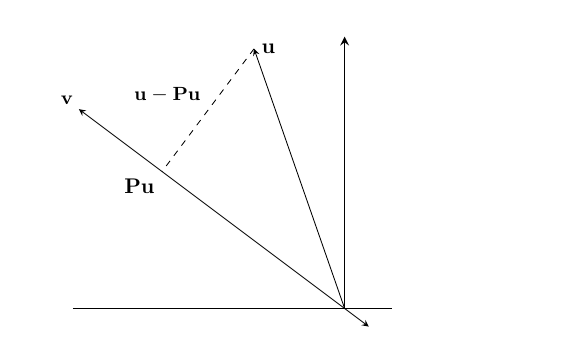
\includegraphics[width=0.4\textwidth,height=\textheight]{Proyecction_Ortogonal.png}
\caption{\(v\) en base canónica}
\end{figure}

\hypertarget{ortogonalizaciuxf3n-de-gramm-schmidt}{%
\subsection{Ortogonalización de
Gramm-Schmidt}\label{ortogonalizaciuxf3n-de-gramm-schmidt}}

Se busca obtener la existencia de una base de vectores ortonormales de
un espacio vectorial. Sabemos que si \(V\) es un espacio vectorial
finitamente generado, entonces existe una base \(\mathcal{B}\). ¿Existe
una base de vectores \emph{ortonormales}?

El proceso de ortogonalización da una respuesta afirmativa y un
procedimiento para calcular una base ortonormal a partir de una base de
vectores.

Sea \(\mathcal{B}=\{v_1,v_2,\ldots,v_n\}\) una base ordenada de \(V\).

Definimos a los siguientes vectores \[
w_1=v_1,
\]

\[
w_2 = v_2 - P_{w_1}w_2 = v_2 - \frac{\langle v_2,w_1 \rangle}{\langle w_1,w_1 \rangle}w_1,
\]

\[
w_{n-1} = v_{n-1} - \sum^{n-2}_{k=1} P_{w_k}v_{n-1} = v_{n-1} - \frac{\langle v_{n-1},w_1 \rangle}{\langle w_1,w_1 \rangle}w_1- \frac{\langle v_{n-1},w_2 \rangle}{\langle w_2,w_2 \rangle}w_2 \ldots - \frac{\langle v_{n-1},w_{n-2} \rangle}{\langle w_{n-2},w_{n-2} \rangle}w_{n-2},
\]

\[
w_{n} = v_{n} - \sum^{n-1}_{k=1} P_{w_k}v_{n} = v_{n} - \frac{\langle v_{n},w_1 \rangle}{\langle w_1,w_1 \rangle}w_1- \frac{\langle v_{n},w_2 \rangle}{\langle w_2,w_2 \rangle}w_2 \ldots - \frac{\langle v_{n},w_{n-1} \rangle}{\langle w_{n-1},w_{n-1} \rangle}w_{n-1},
\]

Posteriormente, la base \textbf{ortonormal}
\(\mathcal{O}=\{\mathbf{y}_1,\mathbf{y}_2,\ldots , \mathbf{y}_n\}\) está
dada por \[
\mathbf{y}_i = \frac{w_i}{\|w_i\|}
\]

\hypertarget{proposiciuxf3n-2}{%
\subsubsection{Proposición}\label{proposiciuxf3n-2}}

Los vectores \(\mathbf{w}_i\) son ortogonales a los vectores
\(\mathbf{w}_1,\mathbf{w}_2,\ldots,\mathbf{w}_{i-1}\). Por hipótesis de
inducción, supondremos que \(\mathbf{w}_{i-1}\) es ortogonal a los
vectores \(\mathbf{w}_1,\mathbf{w}_2,\ldots,\mathbf{w}_{i-2}\), entonces
por la linealidad del producto interno si \(i\ne j\) \[
\langle w_i, w_j \rangle = \biggl< \mathbf{v}_{i} - \sum_{k=1}^{n} \frac{\langle \mathbf{v}_{i}, \mathbf{w}_{k} \rangle}{\|\mathbf{w}_k\|^2}\mathbf{w}_k,\mathbf{w}_j\biggr>= \langle \mathbf{v}_i, \mathbf{w}_j \rangle - \sum_{k=1}^n \frac{\langle \mathbf{v}_{i}, \mathbf{w}_{k} \rangle}{\|\mathbf{w}_k\|^2}\langle \mathbf{w}_k, \mathbf{w}_j \rangle
\] \[
\langle w_i, w_j \rangle = \langle \mathbf{v}_i, \mathbf{w}_j \rangle - 
 \frac{\langle \mathbf{v}_{i}, \mathbf{w}_{j} \rangle}{\|\mathbf{w}_j\|^2}\langle \mathbf{w}_j, \mathbf{w}_j \rangle=0
\]

\hypertarget{teorema.-procedimiento-de-gram-schmidt}{%
\subsubsection{Teorema. Procedimiento de
Gram-Schmidt}\label{teorema.-procedimiento-de-gram-schmidt}}

Suponga que \(v_1,\ldots,v_m\) es una lista de vectores linealmente
independientes en \(V\). Definimos \[
\begin{matrix}
\mathbf{w}_1=\mathbf{v}_1, &\quad\quad & \mathbf{w}_2=\mathbf{v}_2 - \frac{\langle \mathbf{v}_2, \mathbf{w}_1 \rangle}{\|\mathbf{w}_1\|^2}\mathbf{w}_1, \\
 \ldots & \quad\quad & \ldots  \\
\mathbf{w}_m= \mathbf{v}_m - \sum_{k=1}^{m-1}\frac{\langle\mathbf{v}_n, \mathbf{w}_k\rangle}{\|\mathbf{w}_k\|^2}\mathbf{w}_{k}
\end{matrix}
\] \begin{equation}
  \mathbf{y}_i=\frac{\mathbf{w}_i}{\|\mathbf{w}_i\|},\mbox{ para todo }i=1,\ldots,m
\end{equation}

Entonces \(\{\mathbf{u}_1,\mathbf{u}_2,\ldots, \mathbf{u}_m\}\) es una
lista de vectores ortonormales en \(V\). Y además \[
\mathcal{S}(\mathbf{v}_1,\mathbf{v}_2,\ldots, \mathbf{v}_m) = \mathcal{S}(\mathbf{y}_1,\mathbf{y}_2,\ldots, \mathbf{y}_m)
\]

Adicionalmente, esto prueba que todo espacio vectorial con producto
interno tiene una base \emph{ortonormal}.

\hypertarget{teorema}{%
\subsubsection{Teorema}\label{teorema}}

Sea \(V\) un espacio vectorial con producto interno finito-dimensional,
entonces \(V\) tiene una base ortonormal.

\hypertarget{ejemplo}{%
\paragraph{Ejemplo}\label{ejemplo}}

\begin{enumerate}
\def\labelenumi{\alph{enumi})}
\item
  Usar el proceso de ortogonalización de Gram-Schmidt para determinar
  una base ortonormal de \(\mathbb{R}^3\), a partir de los siguientes
  vectores \[
  \begin{Bmatrix}
    \begin{pmatrix}1\\ 1 \\ 0 \end{pmatrix},
    \begin{pmatrix}0\\ 1 \\-1 \end{pmatrix},
    \begin{pmatrix}1\\ 0 \\-1 \end{pmatrix}
  \end{Bmatrix}
  \]
\item
  Usa el proceso de ortogonalización de Gram-Schmidt para determinar una
  base ortogonal a partir de \[
  \begin{Bmatrix}
    \begin{pmatrix} 1\\ 2 \\ 3 \end{pmatrix},
    \begin{pmatrix} 4\\ 5 \\ 0 \end{pmatrix},
    \begin{pmatrix} 2\\ 3 \\-1 \end{pmatrix}
  \end{Bmatrix}
  \]
\item
  Encuentra una base ortonormal para el subespacio generado por los
  vectores \[
  \begin{Bmatrix}
    \begin{pmatrix} 0\\ 2 \\ 1 \end{pmatrix},
    \begin{pmatrix} 1\\ -2 \\ 1 \end{pmatrix}
  \end{Bmatrix}
  \]
\end{enumerate}

Solución a) \[
\mathbf{w}_1=\begin{pmatrix} 1 \\ 1 \\ 0 \end{pmatrix}
\] entonces \[
\mathbf{w}_2=\begin{pmatrix} 0 \\ 1 \\ -1 \end{pmatrix} - \frac{(0,1,-1)\cdot(1,1,0)}{(1,1,0)\cdot (1,1,0)}\begin{pmatrix} 1\\ 1 \\ 0\end{pmatrix} =\begin{pmatrix} 0 \\ 1 \\ -1 \end{pmatrix} - \frac{1}{2}\begin{pmatrix} 1\\ 1 \\ 0\end{pmatrix} =
\begin{pmatrix} -1/2\\ 1/2 \\ -1\end{pmatrix}
\]

\[
\mathbf{w}_3=
\begin{pmatrix} 1 \\ 0 \\ -1 \end{pmatrix} - \frac{(1,0,-1)\cdot(1,1,0)}{(1,1,0)\cdot (1,1,0)}
\begin{pmatrix} 1\\ 1 \\ 0\end{pmatrix}  - \frac{(1,0,-1)\cdot(-1/2,1/2,-1)}{(-1/2,1/2,-1)\cdot(-1/2,1/2,-1)}
\begin{pmatrix} -\frac{1}{2}\\ \frac{1}{2} \\ -1\end{pmatrix} =
\begin{pmatrix} 2/3 \\ -2/3 \\ -2/3\end{pmatrix}
\] Calculamos la norma \[
\begin{matrix} 
  \|w_1\|= & \sqrt{1^2 + 1^2 +0^2}=\sqrt{2} \\
  \|w_2\|= & \sqrt{(-\frac{1}{2})^2 + (\frac{1}{2})^2+ (-1)^2} = \sqrt{\frac{3}{2}}\\
  \|w_3\|= & \sqrt{(\frac{2}{3})^2 + (-\frac{2}{3})^2+ (-\frac{2}{3})^2} = \frac{2}{3}\sqrt{2}
\end{matrix}
\]

\end{document}
